\chapter{Legoblokdetectie op basis van CAD modellen}
\label{hoofdstuk:3}
In het voorgaande hoofdstuk werd een na\"ieve methode aangebracht om legoblokken te detecteren. Deze methode worstelde echter met verschillende nadelen waardoor het (bijna) niet mogelijk was om constructies van legoblokken te detecteren die bestaan uit meerdere niveau's. Om dit soort constructies wel te kunnen detecteren moeten we op zoek naar een meer generiek algoritme dat op basis van alle geometrische informatie een legoblok kan detecteren (zodanig dat de blok kan gevonden worden in eender welke legoconstructie). Daarom wordt in dit hoofdstuk een algoritme behandeld dat op basis van features ge\"extraheerd uit CAD modellen legoblokken kan detecteren in een videoframe.

Eerst leggen we enkele begrippen uit en schetsen we kort het algoritme in sectie \ref{sec:inl_hfdst4}. Vervolgens bespreken we verschillende soorten features voor dit algoritme in sectie \ref{sec:feat} en vergelijken we ze met elkaar in secite \ref{sec:eval_feat}. Ook enkele classificatie methodes voor dit algoritme komen aan bod en worden vergeleken respectievelijk in secties \ref{sec:class} en \ref{sec:eval_class}. Tenslotte geven we in sectie \ref{sec:besl_hfdst4} aan waarom deze methode niet kan worden gebruikt in een AR spel om legoblokken te detecteren.

\section{Begrippen en algoritme} \label{sec:inl_hfdst4}

\subsection{Begrippen}

\begin{figure}
  \centering
  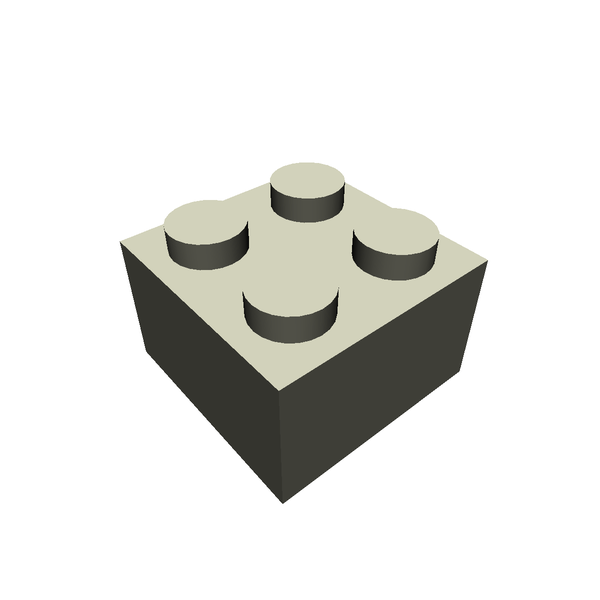
\includegraphics[width=.5\linewidth]{img/cad}
  \caption{Pose van het CAD model van een 2x2 legoblokje.}
  \label{fig:cad}
\end{figure}

\textbf{Computer Aided Design} (CAD) modellen zijn collecties van punten die de geometrie van een 3 dimensionaal object beschrijven, meestal worden ze gebruikt om objecten in een virtuele 3D wereld voor te stellen. Afbeelding \ref{fig:cad} toont een afbeelding van het CAD model van een legoblok dat later in dit hoofdstuk nog wordt gebruikt.

\textbf{Window sliding} is een methode waarbij een rechthoek (het window) geschoven wordt over een afbeelding. Elke keer de rechthoek zich op een nieuwe plaats op de afbeelding bevindt wordt meestal een andere afbeelding vergeleken met het gedeelte van de afbeelding in het window. Deze methode wordt onder andere gebruikt bij object detectie om een object te zoeken in een afbeelding. In dit geval wordt dan, steeds wanneer de rechthoek verschuift, bekeken of het te detecteren object zich in dit window bevindt. Omdat er tijdens window sliding echter geen rekening wordt gehouden met de schaal van het object doen we dit meermaals en wordt de schaal van het window telkens aangepast.

Een \textbf{classifier} is een functie die bij object detectie gebruikt wordt om tijdens window sliding te beslissen of het window het object bevat. In ons geval is de taak van de classifier dus om tijdens het window sliding te beslissen of het window een legoblok bevat.

\textbf{AdaBoost} is een algoritme dat vaak wordt gebruikt in object detectie algoritmes om classifiers sterker te maken tijdens de training. Het idee is dat enkel die zwakke classifiers (die op basis van 1 sample classificeren) worden gekozen die de kleinste trainingsfout maken en deze te combineren tot \'e\'en sterke classifier~\cite{freund1995desicion}. Hier wordt het bij de Haar-like features (zie sectie \ref{sec:feat_haarlike}) ook gebruikt om features te selecteren. 

Een \textbf{integral image} is een afbeelding die gegenereerd wordt van een oorspronkelijke afbeelding door elke pixel vervangen met de som van alle pixels die in de linkerboven rechthoek liggen ten opzichte van de pixel~\cite{viola2001rapid}. Dus indien de pixel in de linkerbovenhoek pixel $(0,0)$ is, dan geldt voor elke pixel in de integral image:
$$p(x,y)=\sum_{x^\prime \leq x,y^\prime \leq y} p(x^\prime,y^\prime)$$

\subsection{Algoritme}
Een CAD model bevat alle geometrische informatie over een object (het moet dat object immers in 3D voorstellen) en dus kan dit model gebruikt worden om een object in een afbeelding te detecteren. Het grote voordeel is dan dat aangezien dit model alle geometrische informatie bevat het object in om het even welke pose kan worden gedetecteerd. Dit is de methode die werd aangebracht in \cite{aubry2014seeing}.

Om CAD modellen te kunnen gebruiken voor object detectie moet eerst nuttig informatie uit deze modellen worden gehaald. In een afbeelding is echter slechts een deel van het object te zien (de afbeelding is namelijk 2D),  daarom is het beter eerst afbeeldingen te genereren van de verschillende poses van het CAD model (figuur \ref{fig:cad} toont een voorbeeld). 

Deze poses bevatten niet het exacte object dat we zoeken in de testafbeelding (het heeft misschien een andere kleur, andere belichting, andere achtergrond, etc.). Daarom moet nog informatie (in vorm van een classifier) ge\"extraheerd worden uit deze afbeeldingen dat we vervolgens kunnen gebruiken voor de detectie. Dit gebeurt tijdens een trainingsfase.

\subsubsection*{Training}
De training bestaat uit het berekenen van een classifier uit een aantal parameters en een hoop positieve en negatieve samples. We hebben ervoor gezorgd dat een deel van de negatieve samples bestaan uit het grondvlak zonder legoblokjes. Hiermee zijn de negatieve samples representatief voor de gebieden waarvan we willen dat ze niet als legoblok worden aanzien (de achtergrond).

De positieve samples zijn opgebouwd uit een set positieve afbeeldingen. Deze set bestaat enerzijds uit de virtueel gegenereerde poses van een 2x2 legoblok en anderzijds uit foto's van zulke legoblok, beide op een witte achtergrond (we gebruiken tijdens detectie immers ook een witte achtergrond). De poses werden gegenereerd van slechts een kwart van de legoblok omdat deze symmetrisch is. De foto's zijn nuttig omdat ze helpen de invloed van belichting op de classifier te minimaliseren aangezien ze werden getrokken in een realistische belichting. 

Tijdens de training wordt een classifier berekend die zo goed mogelijk de positieve samples scheidt van de negatieve samples. Om de verschillende samples met elkaar te kunnen vergelijken worden eerst features berekend van alle samples die we vervolgens kunnen vergelijken met elkaar. Aangezien dit proces afhangt van welke classifier methode wordt gekozen, bespreken we dit uitgebreider in sectie \ref{sec:class}.

\subsection*{Detectie}
Na de training kan met behulp van de gegenereerde classifier en window sliding de legoblok gedetecteerd worden in een testafbeelding. Hiervoor wordt voor elke window de feature vector berekend die vervolgens aan de classifier wordt gegeven. Deze beslist dan of dit window het object bevat of niet.

Omdat de keuze van classifier methode en feature type erg belangrijk is voor het welslagen van dit algoritme worden de verschillende feature types en classifier methodes met elkaar vergeleken in de rest van dit hoofdstuk. De experimenten gebeuren allemaal op een desktop en niet op de smartphone waarop de uiteindelijke legobrick detectie moet worden ge\"implementeerd. Dit is vooral omdat een desktop eenvoudiger is om op te experimenten en omdat het voldoende is om het beste feature type en de beste classificatie methode te bepalen.

\section{Features} \label{sec:feat}

In deze sectie worden drie verschillende soorten features besproken en met elkaar vergeleken: Haar-like~\cite{viola2001rapid}, Multiscale Block Local Binary Patterns~\cite{liao2007learning} (MB-LBP) en Histogram of Oriented Gradients~\cite{dalal2005histograms} (HOG). Tenslotte wordt ook een parts-based feature besproken (gebaseerd op HOG), dat gebruikt werd in \cite{aubry2014seeing}, en waarom deze niet is opgenomen in de evaluatie~\cite{felzenszwalb2010object}.


%In het geval van HOG worden ook twee verschillende methodes voor classificatie met elkaar vergeleken: . Ten slotte wordt kort nog een laatste methode besproken die deels gebaseerd is op HOG~\cite{felzenszwalb2010object}, deze methode zal echter niet worden vergeleken met de andere omdat reeds meermaals werd aangetoond dat deze een te lage performantie heeft om in realtime te gebruiken voor AR.

\subsection{Haar-like} \label{sec:feat_haarlike}
%lienhart2002extended

\begin{figure}
  \centering
  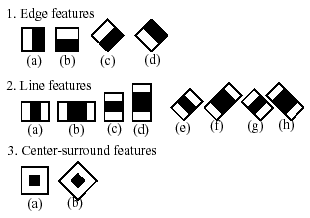
\includegraphics[width=.7\linewidth]{img/haar2}
  \caption{Uitgebreide Haar-like featureset~\cite{lienhart2002extended}.}
  \label{fig:haarUitg}
\end{figure}

Bij de berekening van een Haar-like feature vector wordt het verschil genomen van de som van pixels tussen verschillende rechthoekige regio's. Oorspronkelijk werden vier soorten features gebruikt: twee die elk bestonden uit twee rechthoekige gebieden, \'e\'en soort met drie rechthoekige gebieden en \'e\'en soort met vier rechthoekige gebieden~\cite{viola2001rapid}. Later werden extra features toegevoegd tot de uiteindelijke featureset 14 soorten features bedraagt~\cite{lienhart2002extended}. De uitgebreide featureset is te zien in figuur \ref{fig:haarUitg}: het verschil wordt bepaald door de som te nemen van pixels in de witte regio's en af te trekken van de som van pixels in de zwarte regio's. Alle soorten features zijn eenvoudig uit te rekenen aan de hand van een \textit{integral image} (of een afgeleide daarvan~\cite{lienhart2002extended}).

Om goede features te vinden wordt eerst een enorme hoeveelheid aan features aangemaakt. Aangezien dit aantal features een heel stuk hoger is dan het aantal pixels in het window moet een effici\"ente methode gebruikt worden om de juiste features te selecteren. Hiervoor wordt AdaBoost gebruikt, een methode die origineel wordt gebruikt om een classifier sterker te maken. Aangezien AdaBoost het feature selecteert dat de kleinste fout maakt op de classificatie van positieve en negatieve samples, impliceert dit ook dat elke feature een threshold bevat die aangeeft wanneer deze feature een detectiewindow als juist of onjuist classificeert. De uiteindelijke feature vector van het volledige detectiewindow is de set van de geselecteerde features.

\subsection{MB-LBP} \label{sec:feat_mblbp}

\begin{figure}
  \centering
  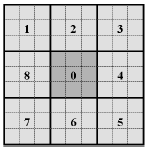
\includegraphics[width=.3\linewidth]{img/lbp}
  \caption{Een 9x9 MB-LBP operator: elk blok bestaat uit 9 pixels~\cite{liao2007learning}.}
  \label{fig:lbp}
\end{figure}

Een MB-LBP feature is een uitbreiding op de originele LBP feature waarin elke pixel werd vergeleken met zijn acht buren. Deze acht buren werden steevast in dezelfde volgorde overlopen en telkens een buur een grotere intensiteit had dan de pixel zelf werd een '1' genoteerd, in de andere gevallen een '0'. Zo wordt voor elke pixel een getal verkregen van acht bits dat de gradi\"ent van de pixel voorstelt in de verschillende richtingen~\cite{ojala1996comparative}.

Hier wordt de MB-LBP feature gebruikt in plaats van de oorspronkelijke LBP omdat deze meer robuust is. In de MB-LBP variant worden, in plaats van een pixel met zijn buren te vergelijken, blokken van pixels met hun buren vergeleken (zie figuur \ref{fig:lbp}). Hierdoor is de feature meer robuust en encodeert het bovendien, naast microstructuren, ook macrostructuren in een afbeelding~\cite{liao2007learning}. 

Om de feature vector van een volledig window te berekenen wordt het window in cellen opgesplitst en vervolgens histogrammen berekend van de MB-LBP features binnen een cel. De histogrammen van alle cellen worden ten slotte aaneengeschakeld om de feature vector te bekomen.

\subsection{HOG} \label{sec:feat_hog}

Bij een HOG feature worden eerst gradi\"enten van alle pixels in een window berekend. Vervolgens wordt het window onderverdeeld in cellen en wordt voor elke cel een histogram van de gradi\"enten gemaakt. Om problemen met belichting en contrast te voorkomen worden cellen gecombineerd tot blokken waarover deze histogrammen worden genormaliseerd. Ten slotte worden alle histogrammen aaneengeschakeld (net als bij MB-LBP) om een feature vector van het window te bekomen~\cite{dalal2005histograms}.

\subsection{Deformed parts-based} \label{sec:feat_part}
Het deformed parts-based feature bestaat uit twee onderdelen: een HOG feature van de volledige window (root filter) en aantal kleinere HOG features van een subwindow (part filters). Deze verschillende part filters worden gedefinieerd door een anker punt ten opzichte van de plaats van de root filter en een functie die alle mogelijke plaatsen van deze part filter beschrijft relatief ten opzichte van het anker punt. De score van de hypothese dat een window het te detecteren object bevat wordt berekend door de sommatie te nemen van de verschillen (voor elke filter) tussen de score van een filter (HOG feature) en een kost voor de vervorming van de filter. Dit model maakt het HOG feature een stuk meer flexibel voor vervormingen of andere poses van een object ~\cite{felzenszwalb2010object}.

Een groot nadeel van deze methode is dat ze nogal wat rekenwerk vraagt om uit te voeren en dus ongeschikt is voor gebruik in real time. Dit probleem is eerder al aangehaald in andere state-of-the-art papers die de performantie hebben kunnen verhogen. Hoewel bijvoorbeeld in paper \cite{yan2014fastest} wordt aangegeven dat 40 FPS haalbaar is, is dit slechts na parallellisatie (over zes threads) en bovendien op een desktop computer. De desktop die in deze recente paper werd gebruikt heeft een 2.66GHz Hexacore Intel X5650 CPU. Dit is een heel stuk krachtiger dan de smartphone (met een 1GHz Quadcore Qualcomm Snapdragon S4 Pro APQ8064 ) die wij uiteindelijk willen gebruiken om het volledige algoritme op te implementeren. Het zou dus erg moeilijk zijn en bovendien veel tijd vragen om dit optimaal te implementeren op de smartphone. Dit verklaart waarom dit feature type voor ons geen interessante piste was en waarom deze niet is opgenomen in onze feature evaluatie.

\section{Evaluatie features} \label{sec:feat_eval_res}
Deze sectie behandelt de evaluatie van de feature types. Eerst wordt kort besproken hoe de evaluatie verloopt en vervolgens worden alle soorten features vergeleken op vlak van robuustheid en performantie.

\subsection{Evaluatiemethode} \label{sec:eval_feat}
De evaluatie van de verschillende features gebeurt door eerst een classifier te trainen voor alle features en vervolgens de geleerde classifiers te gebruiken voor detectie. 

\begin{table}

%\parbox{.45\linewidth}{
	\centering
  	\begin{tabular}{@{}ll@{}} \toprule
    %\cmidrule(r){2-2}
    Parameter & Waarde\\ \midrule
    \textbf{Training} & \\ 
    \# classif. in cascade & 20 \\
    Wind. size & 64x64 \\
    Min. hit rate & 0.999 \\
    Max. false alarm rate & 0.5 \\
    Mode (Haar-like) & ALL \\ \midrule
    \textbf{Detectie} & \\ %\cmidrule(r){2-2}
%    Parameter & Waarde\\ \midrule
    Schaalfactor & 1.1 \\
    Min. \# buren & 15 \\
    Min. grootte & 10x10 (px) \\
    Max. grootte & 100x100 (px) \\ \bottomrule
  \end{tabular}
  \caption{Parameters gebruikt tijdens training en detectie van features met cascade classificatie als classificatie methode.}
  \label{tab:param_ccla}
%}
%\hfill
%\parbox{.45\linewidth}{
%	\centering
%  	\begin{tabular}{@{}ll@{}} \toprule
%    %\cmidrule(r){2-2}
%    Parameter & Waarde\\ \midrule
%    \textbf{Training} & \\ 
%    Padding (HOG) & 0x0 (px) \\
%    Wind. stride (HOG) & 8x8 (px) \\
%    Wind. size (HOG) & 64x64 (px) \\ \midrule
%    \textbf{Detectie} & \\ %\cmidrule(r){2-2}
%%    Parameter & Waarde\\ \midrule
%	Schaalfactor & 1.1 \\
%	Hit threshold & 0.4 \\
%    Padding (HOG) & 0x0 (px) \\
%    Wind. stride (HOG) & 8x8 (px) \\
%    Wind. size (HOG) & 64x64 (px) \\ \bottomrule
%  \end{tabular}
%  \caption{Parameters gebruikt tijdens training en detectie van features met SVM als classificatie methode.}
%  \label{tab:param_svm}
%}
\end{table}

%Voor de \textbf{training} werden ongeveer even veel positieve als negatieve samples gebruikt: de positieve samples begon met een set van 128 afbeeldingen die via transformaties werd vergroot tot 3000 samples. 

\subsubsection*{Training}

Bij de training werden de features steeds getraind tot een cascade classifier (zie sectie \ref{sec:class_ccla}), dit om geen invloed op de resultaten te krijgen door een andere keuze in classificatie methode. Om de training uit te voeren werd gebruik gemaakt van het programma \texttt{opencv\_traincascade}, dat deel is van de OpenCv bibliotheek. Er werden ongeveer even veel positieve als negatieve samples gebruikt: de positieve samples begon met een set van 128 afbeeldingen die via transformaties op een willekeurig gekozen negatieve achtergrond (uit de negatieve samples) werd vergroot tot 3000 samples. Deze transformaties helpen dus om een groter aantal positieve samples te bekomen maar ook om het effect van belichting en rotaties van legoblokken kleiner te maken. 

Omdat de training erg lang kan duren werd deze maar eenmaal uitgevoerd per soort feature om toch een groffe indicatie te geven van hoe lang zulke training duurt. De parameters die tijdens de training werden gebruikt zijn aangegeven in tabel \ref{tab:param_ccla}. 

De training werd uitgevoerd op een machine met een 2.4 GHz CPU met 12 cores en 47GB RAM. Dit is niet dezelfde machine als gebruikt wordt tijdens de detectie omdat die machine veel te traag is om de training op uit te voeren. Bovendien is het niet nuttig om performantie van de training en detectie met elkaar te vergelijken omdat deze waarden ver uit elkaar liggen.

%Bij de vergelijking tussen de classificatie methodes werd steevast voor de HOG features gekozen om dezelfde reden (zie sectie \ref{sec:feat_hog}).

\begin{figure}
\begin{tabular}{cccc}
  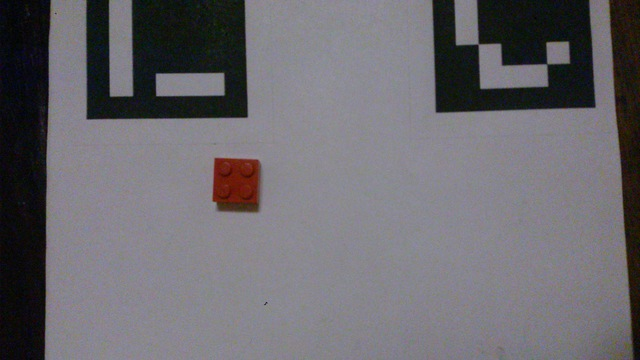
\includegraphics[width=0.25\linewidth]{img/classTestImg/01_top} &   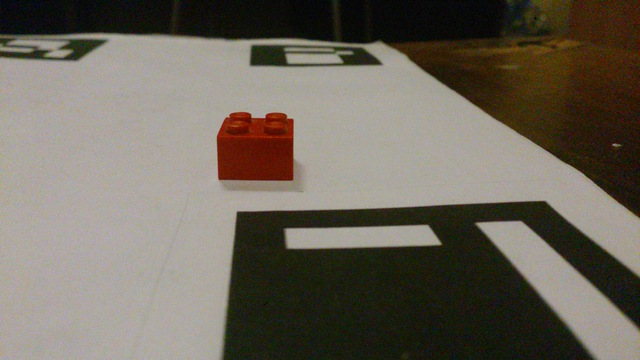
\includegraphics[width=0.25\linewidth]{img/classTestImg/02_side} & 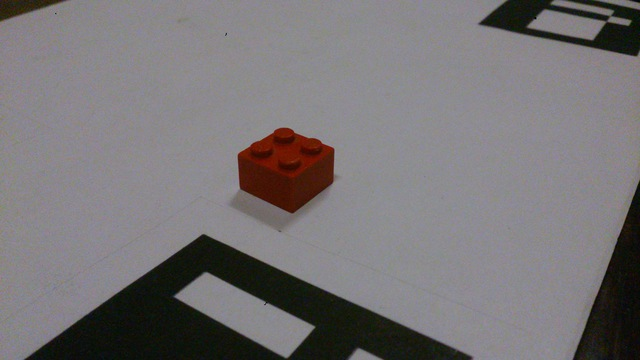
\includegraphics[width=0.25\linewidth]{img/classTestImg/03_persp} &
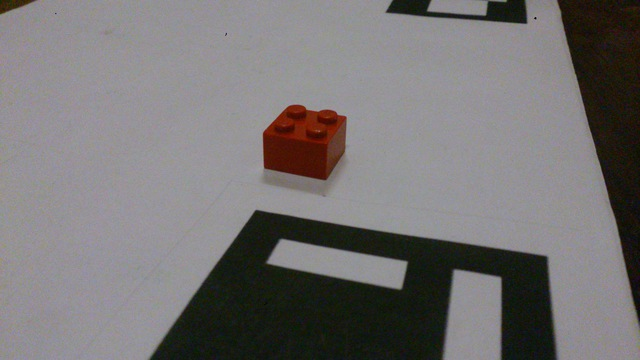
\includegraphics[width=0.25\linewidth]{img/classTestImg/04_rand} \\
  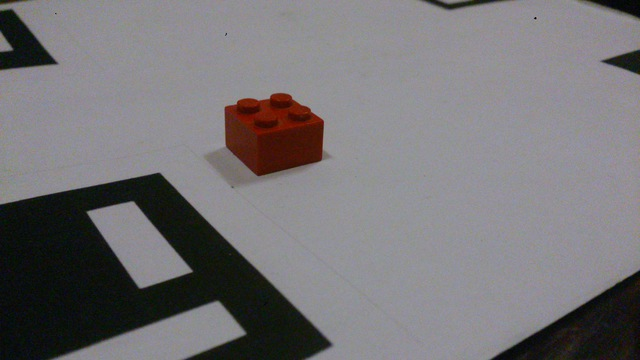
\includegraphics[width=0.25\linewidth]{img/classTestImg/05_rand} &   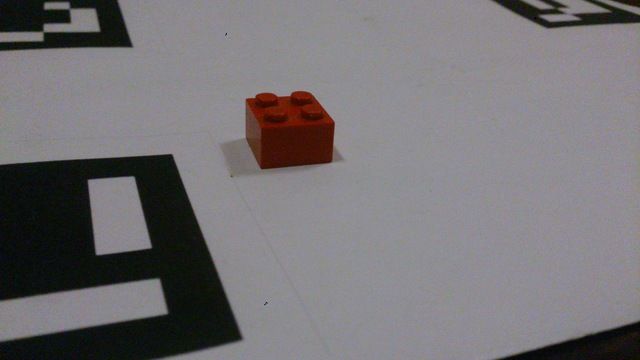
\includegraphics[width=0.25\linewidth]{img/classTestImg/06_rand} & 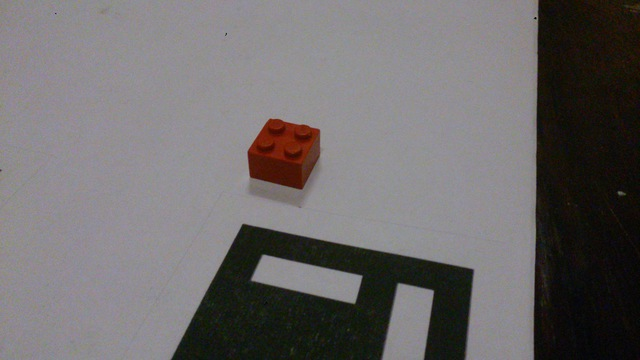
\includegraphics[width=0.25\linewidth]{img/classTestImg/07_rand} &
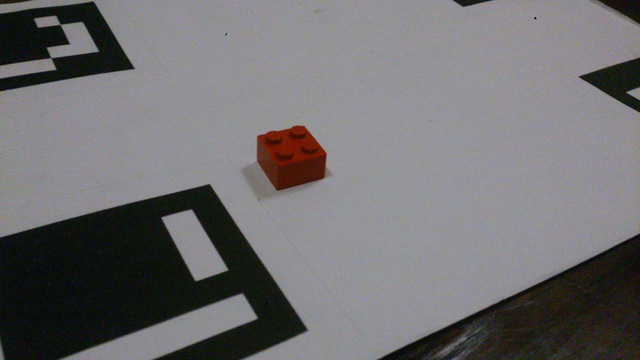
\includegraphics[width=0.25\linewidth]{img/classTestImg/08_rand} \\
  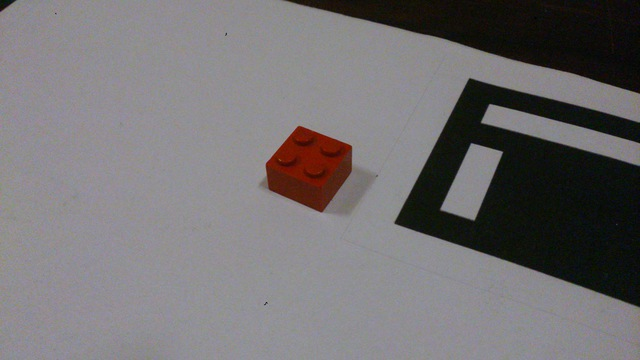
\includegraphics[width=0.25\linewidth]{img/classTestImg/09_rand} &   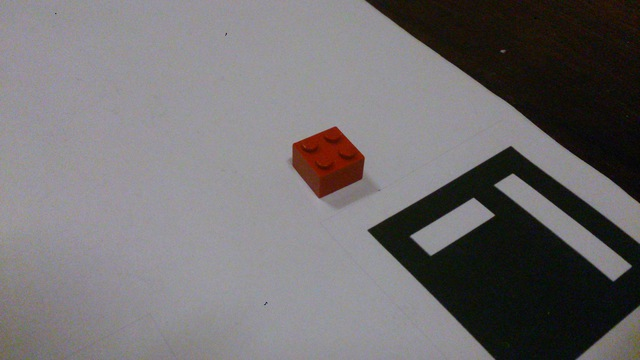
\includegraphics[width=0.25\linewidth]{img/classTestImg/10_rand} & 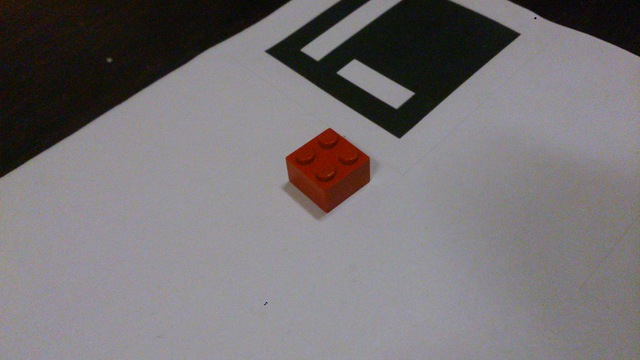
\includegraphics[width=0.25\linewidth]{img/classTestImg/11_rand} &
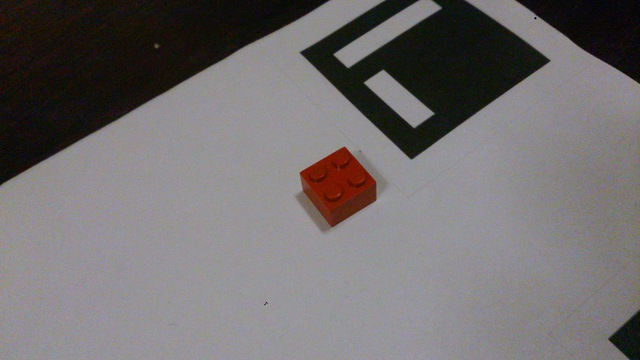
\includegraphics[width=0.25\linewidth]{img/classTestImg/12_rand} \\
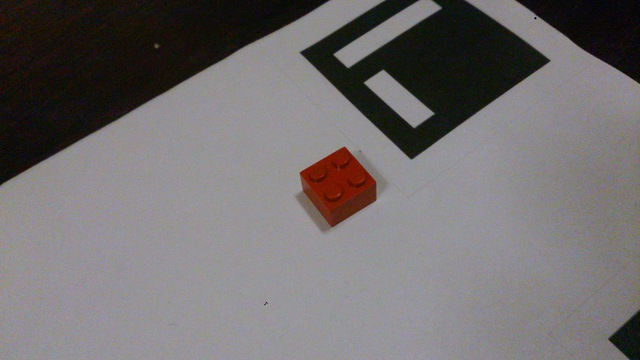
\includegraphics[width=0.25\linewidth]{img/classTestImg/12_rand} &   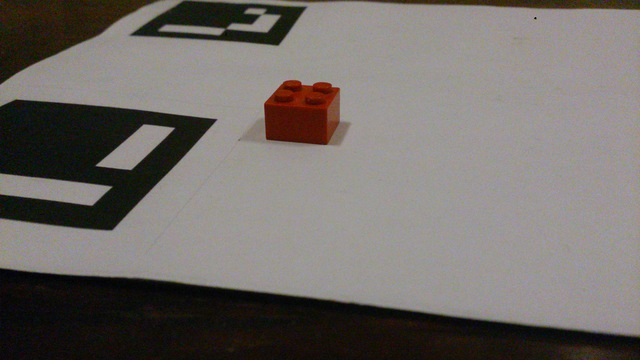
\includegraphics[width=0.25\linewidth]{img/classTestImg/14_rand} & 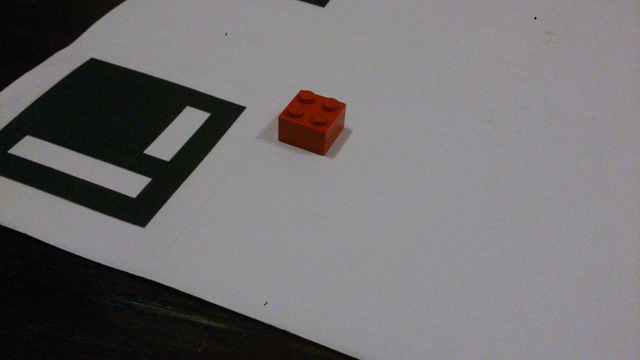
\includegraphics[width=0.25\linewidth]{img/classTestImg/15_rand} &
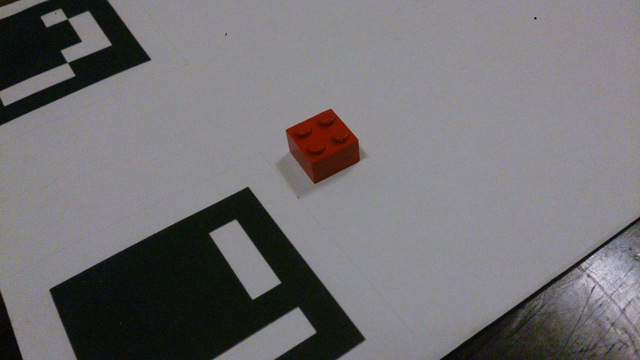
\includegraphics[width=0.25\linewidth]{img/classTestImg/16_rand} \\
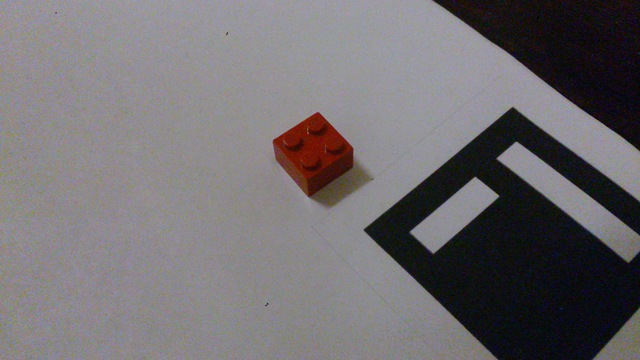
\includegraphics[width=0.25\linewidth]{img/classTestImg/17_rand} &   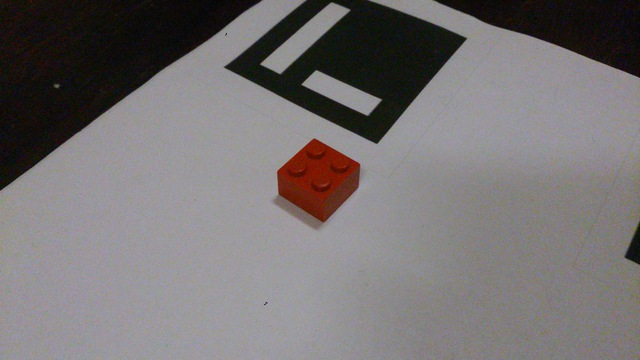
\includegraphics[width=0.25\linewidth]{img/classTestImg/18_rand} & 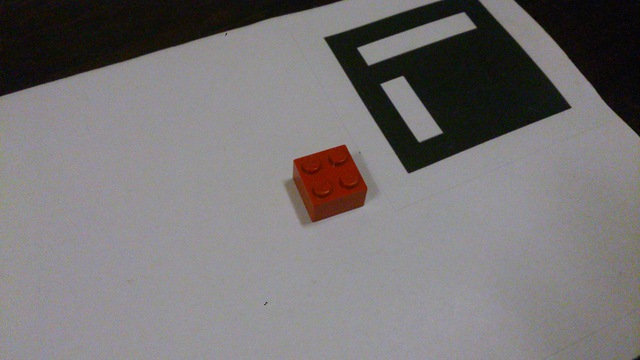
\includegraphics[width=0.25\linewidth]{img/classTestImg/19_rand} &
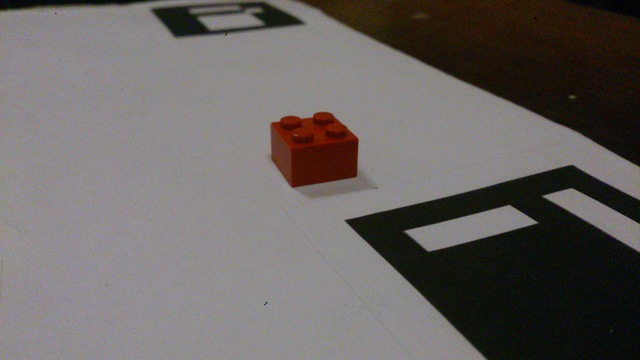
\includegraphics[width=0.25\linewidth]{img/classTestImg/20_rand} \\
%(a) first & (b) second \\[6pt]
% \includegraphics[width=65mm]{it} &   \includegraphics[width=65mm]{it} \\
%(c) third & (d) fourth \\[6pt]
%\multicolumn{2}{c}{\includegraphics[width=65mm]{it} }\\
%\multicolumn{2}{c}{(e) fifth}
\end{tabular}
\caption{De 20 afbeeldingen die als testset werden gebruikt.}
\label{fig:testset}
\end{figure}

\subsubsection*{Detectie}

De detectie gebeurt op 20 afbeeldingen van een legoblok in verschillende poses. Hierbij werden 3 standaardposes gekozen: bovenaanzicht, zijaanzicht en een aanzicht waarin de legoblok vanuit een hoekpunt wordt gezien. De rest van de poses zijn allemaal willekeurig gekozen. Deze afbeeldingen zijn te zien in figuur \ref{fig:testset}: de drie afbeeldingen in links in de eerste rij zijn de drie specifiek gekozen aanzichten, de rest zijn de willekeurige. Deze keuze van poses zal een idee geven over hoe robuust / performant de features zijn tegen wijzigingen in pose en welke poses robuuster / performanter zijn dan andere. De parameters die gebruikt werden tijdens de detectie zijn ook aangegeven in tabel \ref{tab:param_ccla}.

Bij het vergelijken van features zal naar performantie en robuustheid worden gekeken. Voor de experimenten die focussen op performantie werd de detectie 10x uitgevoerd op alle 20 testafbeeldingen en per afbeelding het gemiddelde genomen.

De experimenten werden uitgevoerd op een \textbf{machine} met een Intel Core 2 Duo 2,4 GHz processor, een NVIDIA GeForce 320M 256 MB grafische kaart, 8 Gb RAM en Mac OS X 10.10.2. Alle implementaties zijn geschreven in C++ en maken gebruik van OpenCV 2.4.9.

\subsection{Vergelijking}
In deze sectie worden de eerste drie besproken feature types met elkaar vergeleken. Ze worden vergeleken qua performantie en robuustheid.

%\paragraph{Eigenschappen}

%\begin{table}
%  \centering
%  \begin{tabular}{@{}lccc@{}} \toprule
%    & \multicolumn{3}{c}{Features} \\ \cmidrule(r){2-4}
%    & Haar-like & MB-LBP & HOG\\ \midrule
%    Berekening & Snel & Snel & Traag \\
%    Occlusie & Neen & Neen & Neen \\
%    Scope & Lokaal & Globaal & Globaal \\\bottomrule
%  \end{tabular}
%  \caption{Feature eigenschappen.}
%  \label{tab:feat_eig}
%\end{table}
%
%In tabel \ref{tab:feat_eig} worden een aantal eigenschappen opgesomd, waarin de verschillende soorten features met elkaar worden vergeleken. 
%
%De berekening van Haar-like en MB-LBP features is snel, omdat dit kan door gebruik te maken van integraal afbeeldingen~\cite{viola2001rapid}. HOG is ten opzichte van Haar-like en MB-LBP features echter 
%
%Zowel bij Haar-like als bij MB-LBP features kan AdaBoost gebruikt worden om een krachtige classifier te construeren.

\subsubsection*{Performantie}

\begin{figure}
  \centering
  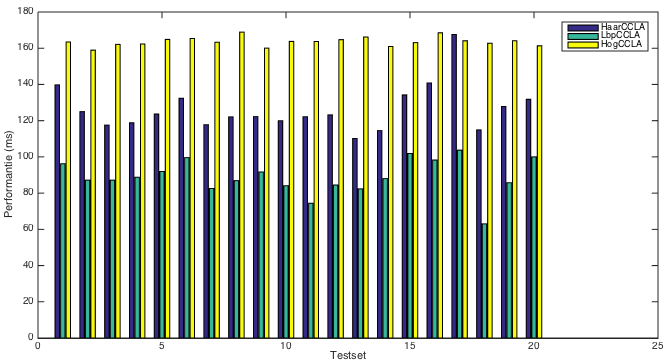
\includegraphics[width=\linewidth]{img/FeaturePerf}
  \caption{Feature performantie tijdens detectie.}
  \label{fig:featPerf}
\end{figure}

De vergelijking van performantie tussen verschillende soorten features bestaat uit twee onderdelen: enerzijds de snelheid bij training van de classifier en anderzijds de snelheid bij detectie.

De duur van de training wordt aangegeven in tabel \ref{tab:feat_perf}. Het is belangrijk op te merken dat tijdens de HOG training slechts 1 core wordt gebruikt terwijl de andere soorten alle CPU cores gebruikten, dit is inherent aan de implementatie van OpenCV. We kunnen er wel uit afleiden dat HOG waarschijnlijk snelle kan worden getraind dan MB-LBP indien alle cores werden gebruikt. Het opmerkelijkste is het groot verschil is tussen de tijd nodig om een Haar-like classifier te trainen en tijd nodig om een LBP of HOG classifier te trainen. Dit valt als volgt te verklaren: bij het trainen van een Haar-like classifier wordt eerst voor elke window een enorme hoeveelheid aan features gegenereerd die vervolgens worden uitgeselecteerd met AdaBoost~\cite{freund1995desicion}. Deze hoeveelheid aan features is vele malen groter dan het aantal pixels in het window, in tegenstelling tot MB-LBP en HOG waarbij voor elk window enkel een aantal histogrammen worden opgesteld.

De performantie tijdens detectie van de 20 testafbeeldingen wordt weergegeven in figuur \ref{fig:featPerf}. Het is duidelijk dat MB-LBP de snelste is, dit komt omdat bij MB-LBP integerwaarden worden vergeleken terwijl bij de rest floating point getallen worden vergeleken. Haar-like is bovendien sneller dan HOG, wat valt te verklaren door het feit dat aan Haar-like een intensieve training vooraf gaat waarna specifieke features zijn geselecteerd die eenvoudig te berekenen zijn via een \textit{integral image}. Bij HOG  moet tijdens de detectie voor elk window een volledig histogram worden berekend wat rekenintensiever is dan het uitrekenen een beperkte set van eenvoudig te berekenen features.

\begin{table}
  \centering
  \begin{tabular}{@{}lcc@{}} \toprule
    Feature & Training & \# cores\\ \midrule
	Haar-like & > 4 dagen & 12 \\
	MB-LBP & $\pm$ 2h & 12\\
	HOG & $\pm$ 3h & 1\\ \bottomrule
  \end{tabular}
  \caption{Feature training tijdsduur.}
  \label{tab:feat_perf}
\end{table}

\subsubsection*{Robuustheid}

Uit de resultaten van figuur \ref{fig:featRobuust} kan worden afgeleid dat detectie met behulp van HOG de beste resultaten geeft: geen enkele afbeelding uit de testset was vals positief en op 4 afbeeldingen uit de testset na werd de legoblok overal correct gevonden. Hoewel met MB-LBP alle legoblokken werden gevonden, vertoont het heel wat meer valse positieven. Haar-like ligt tussen beide in: het detecteert \'e\'en legoblok meer als HOG maar heeft wel twee valse positieven, terwijl HOG er geen enkele heeft.

\begin{figure}
  \centering
  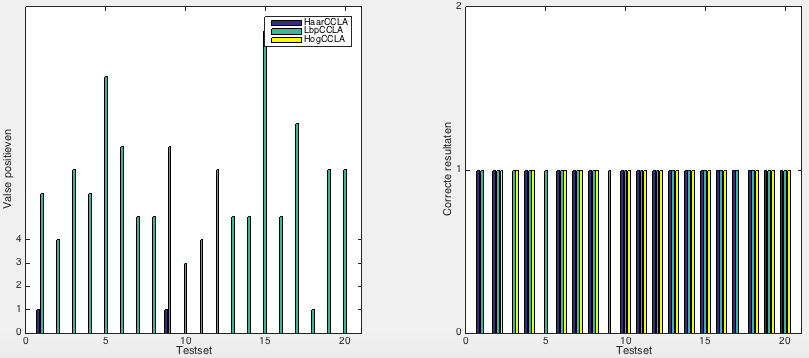
\includegraphics[width=\linewidth]{img/FeatRobust}
  \caption{Feature robuustheid.}
  \label{fig:featRobuust}
\end{figure}

\subsection{Besluit}
We kunnen besluiten dat HOG het meest robuuste feature type is maar dat MB-LBP een stuk sneller. Ook is belangrijk dat hoewel Haar-like features redelijk robuust en performant zijn, er erg veel tijd in kruipt om ze trainen.

\section{Classificatie methodes} \label{sec:class}
Deze sectie behandelt de classificatie methodes. De taak van de classificatie methodes is om op basis van berekende features een legoblok te detecteren. De volgende classificatie methodes besproken: Cascade Classifiers \cite{viola2001rapid} (CCLA) en Support Vector Machines~\cite{joachims1999svmlight} (SVM).

\subsection{CCLA} \label{sec:class_ccla}
Bij een \textbf{CCLA} wordt een classifier getraind door een aantal feature classifiers te combineren. Elk van deze classifiers bestaat uit een aantal features op basis waarvan elke subwindow van een frame wordt geclassificeerd. Zulke cascade classifier werkt door eerst elke subwindow van de frame te laten evalueren door de eerste classifier, indien de eerste classifier de subwindow aanvaardt triggert dit een evaluatie door de volgende classifier in de cascade. Enkel wanneer een window door alle classifiers is aanvaard, kan er vanuit worden gegaan dat dit window het te detecteren object bevat. Door een cascade van classifiers te gebruiken moet elke classifier van de cascade niet al te sterk zijn waardoor negatieve windows al sneller kunnen worden afgevoerd, wat de detectie des te sneller maakt.

\subsection{SVM} \label{sec:class_svm}
Een \textbf{SVM} classificeert op een andere manier: elk subwindow wordt voorgesteld als een p-dimensionale vector in een p-dimensionale ruimte. Met behulp van (p-1)-dimensionale hyperplane worden de subwindows gesplitst in twee groepen: de ene groep wordt aanvaard, de andere niet. De \textit{hit threshold} parameter bepaald hoe ver een vector van de hyperplane moet liggen om te worden aanvaard of afgekeurd. Deze lineaire classifier was het oorspronkelijke algoritme~\cite{vapnik1963pattern}, later werd ook een methode ontwikkelt voor non-lineaire classificatie~\cite{boser1992training}.

\section{Evaluatie classifier methodes} \label{sec:class_eval_res}
Deze sectie behandelt de evaluatie van de classifier methodes. Eerst wordt kort besproken hoe de evaluatie verloopt, vervolgens worden beide methodes (CCLA en SVM) vergeleken op vlak van robuustheid en performantie. Ten slotte wordt de impact bekeken van de \textit{schaalfactor} parameter op robuustheid en performantie voor zowel CCLA als SVM.

\subsection{Evaluatiemethode} \label{sec:eval_class}
De evaluatie van de verschillende classifier methodes gebeurt door elke soort classifier te trainen voor \'e\'en bepaalde feature en vervolgens de geleerde classifiers te gebruiken voor detectie. 

\begin{table}
%\parbox{.45\linewidth}{
	\centering
  	\begin{tabular}{@{}ll@{}} \toprule
    %\cmidrule(r){2-2}
    Parameter & Waarde\\ \midrule
    \textbf{Training} & \\ 
    Padding (HOG) & 0x0 (px) \\
    Wind. stride (HOG) & 8x8 (px) \\
    Wind. size (HOG) & 64x64 (px) \\ \midrule
    \textbf{Detectie} & \\ %\cmidrule(r){2-2}
%    Parameter & Waarde\\ \midrule
	Schaalfactor & 1.1 \\
	Hit threshold & 0.4 \\
    Padding (HOG) & 0x0 (px) \\
    Wind. stride (HOG) & 8x8 (px) \\
    Wind. size (HOG) & 64x64 (px) \\ \bottomrule
  \end{tabular}
  \caption{Parameters gebruikt tijdens training en detectie van features met SVM als classificatie methode.}
  \label{tab:param_svm}
%}
\end{table}

\subsubsection*{Training}

Bij de vergelijking tussen de classificatie methodes werd steevast voor de HOG features (zie sectie \ref{sec:feat_hog}) gekozen om geen invloed op de resultaten te krijgen door een andere keuze in features. Om de training uit te voeren werd gebruik gemaakt van het programma \texttt{opencv\_traincascade} (van de OpenCv bibliotheek) om een CCLAclassifier te trainen en van de SVMLight bibliotheek~\cite{joachims1999svmlight} om een SVM classifier te trainen. Als positieve samples werd de oorspronkelijke set van 128 afbeeldingen gebruikt en als negatieve samples werden dezelfde afbeeldingen gebruikt als bij de features (maar ze werden wel opgesplitst in tiles van 64x64 omdat de implementatie van SVMLight dat vereist).

Opnieuw werd training maar eenmaal uitgevoerd per classifier methode om een groffe indicatie te geven van hoe lang zulke training duurt. De parameters die tijdens de training werden gebruikt zijn aangegeven in tabellen \ref{tab:param_ccla} en \ref{tab:param_svm} voor CCLA en SVM respectievelijk. 

De training werd opnieuw uitgevoerd op een machine met een 2.4 GHz CPU met 12 cores en 47GB RAM, vanwege dezelfde reden als bij de feature evaluatie.

\subsubsection*{Detectie}

De detectie gebeurt, net als bij features, op 20 afbeeldingen van een legoblok in verschillende poses. Deze afbeeldingen zijn te zien in figuur \ref{fig:testset}: de drie afbeeldingen in rechts in de eerste rij zijn de drie specifiek gekozen aanzichten, de rest zijn de willekeurige. De parameters die gebruikt werden tijdens de detectie zijn ook aangegeven in tabellen \ref{tab:param_ccla} en \ref{tab:param_svm}.

Bij het vergelijken van classifier methodes zal naar performantie, robuustheid en de impact van de schaalfactor op de performantie en robuustheid worden gekeken. Voor de experimenten die focussen op performantie werd de detectie 10x uitgevoerd op alle 20 testafbeeldingen en per afbeelding het gemiddelde genomen. In het geval van experimenten met de schaalfactor wordt bij de performantie het gemiddelde genomen over alle testafbeeldingen.

De experimenten werden, net als bij de features, uitgevoerd op een machine met een Intel Core 2 Duo 2,4 GHz processor, een NVIDIA GeForce 320M 256 MB grafische kaart, 8 Gb RAM en Mac OS X 10.10.2. Alle implementaties zijn geschreven in C++ en maken gebruik van OpenCV 2.4.9 (zowel training als detectie).

\subsection{Evaluatie}

\subsubsection*{Robuustheid}

Figuur \ref{fig:classRobuust} toont de robuustheid van de twee classifier methodes. Merk op dat de grafiek met valse positieven is weggelaten omdat deze in beide gevallen overal nul was. We merken op dat de robuustheid van de SVM hoger ligt dan die van de CCLA. De oorzaak hiervan dat SVM alle features gebruikt om die lineair te classificeren, terwijl CCLA slechts een subset van alle features gebruikt om een zo klein mogelijke fout te maken op de classificatie.

\begin{figure}
  \centering
  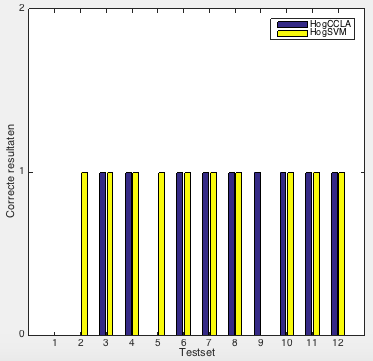
\includegraphics[width=0.75\linewidth]{img/ClassRobust}
  \caption{Robuustheid classifier methodes.}
  \label{fig:classRobuust}
\end{figure}

\subsubsection*{Performantie}

\begin{figure}
  \centering
  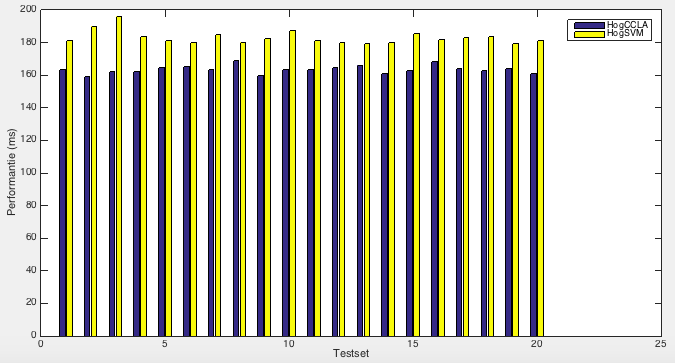
\includegraphics[width=\linewidth]{img/ClassPerf}
  \caption{Classifier methodes performantie tijdens detectie.}
  \label{fig:class_perf}
\end{figure}

De vergelijking van performantie tussen verschillende soorten classificatie methodes bestaat uit twee onderdelen: enerzijds de snelheid bij training van de classifier en anderzijds de snelheid bij detectie.

De duur van de training wordt aangegeven in tabel \ref{tab:feat_perf}. Dit geeft aan dat een SVM classifier een heel stuk sneller kan getraind worden dan een CCLA classifier. Dit komt omdat de SVM classifier features moet uitrekenen en een hyperplane bepalen tussen de features. CCLA, daarentegen, moet een hele cascade van classifiers opbouwen waarbij telkens opnieuw goede features moeten worden gekozen, dit vraagt heel wat meer rekenwerk.

De performantie tijdens detectie van de 20 testafbeeledingen wordt weergegeven in figuur \ref{fig:featPerf}. Dat de detectie langer duurt bij een SVM is logisch aangezien het een lineaire classifier is war vergeleken kan worden met \'e\'en enkele classifier uit een cascade. Om een voldoende goede detectie te behalen moet een SVM dus erg correct kunnen classificeren, dit vergt meer tijd aangezien een cascade juist is ontwikkeld om effici\"enter te zijn dan een enkele classifier.

\begin{table}
  \centering
  \begin{tabular}{@{}lcc@{}} \toprule
    Feature & Training & \# cores \\ \midrule
    CCLA & $\pm$ 3h & 1\\
    SVM & TODO & 1\\ \bottomrule
  \end{tabular}
  \caption{Classifier methodes training tijdsduur.}
  \label{tab:class_perf}
\end{table}

\subsubsection*{Schaalfactor}
De schaalfactor is een parameter die bepaalt hoe sterk de schaal van het window wordt gewijzigd tussen een minimum en maximum grootte. Dus wanneer deze kleiner wordt zullen normaal gezien meer iteraties nodig zijn, terwijl een nauwkeurigere detectie plaatsvindt.

Om de impact van de schaalfactor te bepalen, wordt de performantie en robuustheid van de HOG feature opgemeten wanneer de schaalfactor 1.01, 1.05, 1.10, 1.15, ... , 4 bedraagt. Uit figuur \ref{fig:featScale} is het duidelijk dat aan de verwachtingen voldaan is: de performantie (rechts) is hoger (het aantal ms daalt) bij een hogere schaalfactor, terwijl het aantal correcte detecties (links) daalt. Het aantal valse positieven werd ook gemeten maar deze was voor beide classifiers bijna altijd 0. 

Bij de grafiek die het \textbf{aantal correcte detecties} toont zien we dat in het begin SVM robuuster is dan CCLA, daarna wisselt het wat af.

Dat het aantal correcte poses in het begin hoger ligt bij SVM dan bij CCLA terwijl zijn performantie over het algemeen hoger ligt kan op dezelfde manier verklaard worden als bij de performantie is geredeneerd. Vanwege het lineaire karakter van een SVM is het dan ook logisch dat wanneer een hogere robuustheid wordt gehaald (in het begin) de performantie lager ligt. 

Het wisselend karakter van de eerste grafiek ligt aan de aard van de parameter: indien de schaalfactor toevallig een waarde heeft waardoor het window even groot wordt als een bepaalde legoblok zal deze worden gedetecteerd. Merk op dat deze eerste grafiek slechts tot 1.65 wordt getoond, dit komt omdat het aantal correcte detecties hierna toch steeds 0 is. Dat het reeds bij 1.65 altijd 0 is, komt omdat wanneer de schaalfactor te hoog wordt slechts enkele verschillende groottes als window worden gebruikt. Indien de groottes van deze windows niet toevallig dicht genoeg liggen bij de grootte van de legoblok zal deze niet gedetecteerd worden.

Opmerkelijk is de vorm van de grafiek die de \textbf{performantie} toont, het geeft aan dat beide classifier methodes een performantie hebben van de orde $O(1/(s-1))$ met $s$ de schaalfactor. Merk op dat de orde $1/(s-1)$ is en niet $1/s$ omdat de verticale asymptoot moet liggen op $s = 1$ want als de schaalfactor 1 is duurt de detectie oneindig lang, het window wordt dan immers niet groter.

\begin{figure}
  \centering
  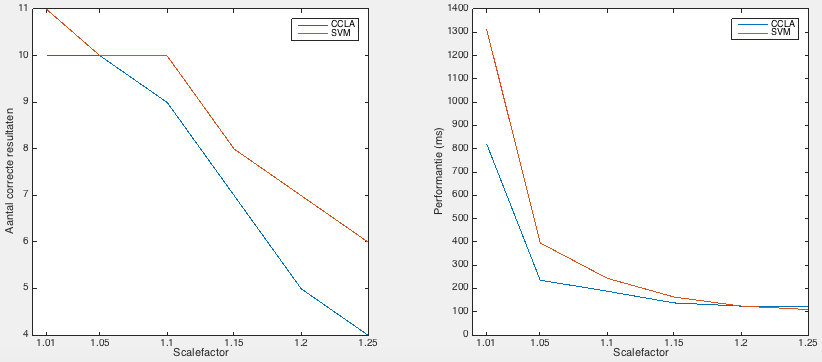
\includegraphics[width=\linewidth]{img/scaleFact}
  \caption{Impact schaalfactor op performantie en robuustheid van HOG feature.}
  \label{fig:featScale}
\end{figure}

\subsection{Besluit}
In deze evaluatie werd aangetoond dat SVM een meer robuustere methode is dan CCLA, maar dat CCLA wel de meer performante is. Vervolgens werd aangetoond dat een hogere schaalfactor de performantie verhoogt maar de robuustheid verlaagt. Tenslotte werd duidelijk dat de performantie van beide methodes van orde $O(1/(s-1))$ is met $s$ de schaalfactor.


\section{Discussie / Besluit} \label{sec:besl_hfdst4}

\begin{figure}
  \centering
  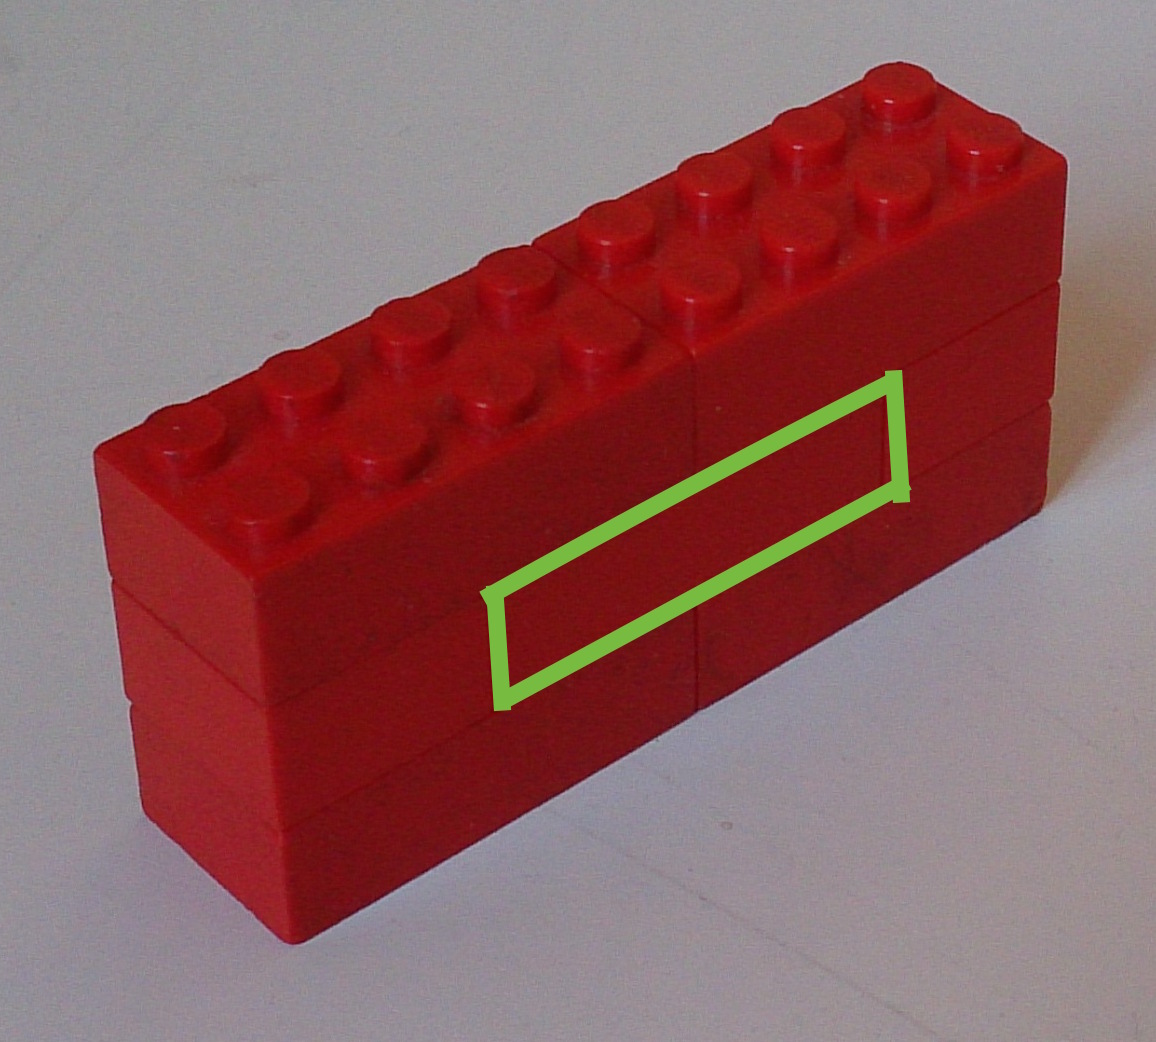
\includegraphics[width=0.5\linewidth]{img/brickWall}
  \caption{Een voorbeeld van een legoblokconstructie waarin het groen omlijnde vlak het enige is wat we van die legoblok zien.}
  \label{fig:brickWall}
\end{figure}

In dit hoofdstuk werd onderzocht welke feature types en classifier methodes beter werken voor detectie van legoblokken. Zo is aangetoond dat HOG de meer robuuste feature type is en dat MB-LBP de meest performante van de drie is. Verder werd aangegeven dat een vierde type feature (op basis van deformed parts-based modellen) te traag is om nuttig te gebruiken in een AR applicatie. Ten slotte toonde de vergelijking tussen classifier methodes aan dat detectie met een SVM classifier vaak trager is maar tegelijk ook meer robuust , dat een hogere schaalfactor leidt tot hogere performantie maar lagere robuustheid en dat de performantie van de classifier methodes van orde $1/(s-1)$ is met $s$ de schaalfactor. De methode die in dit hoofdstuk werd onderzocht is echter niet nuttig om te gebruiken in een AR spel om legoblokken te detecteren en hier is waarom:

\begin{figure}
  \centering
  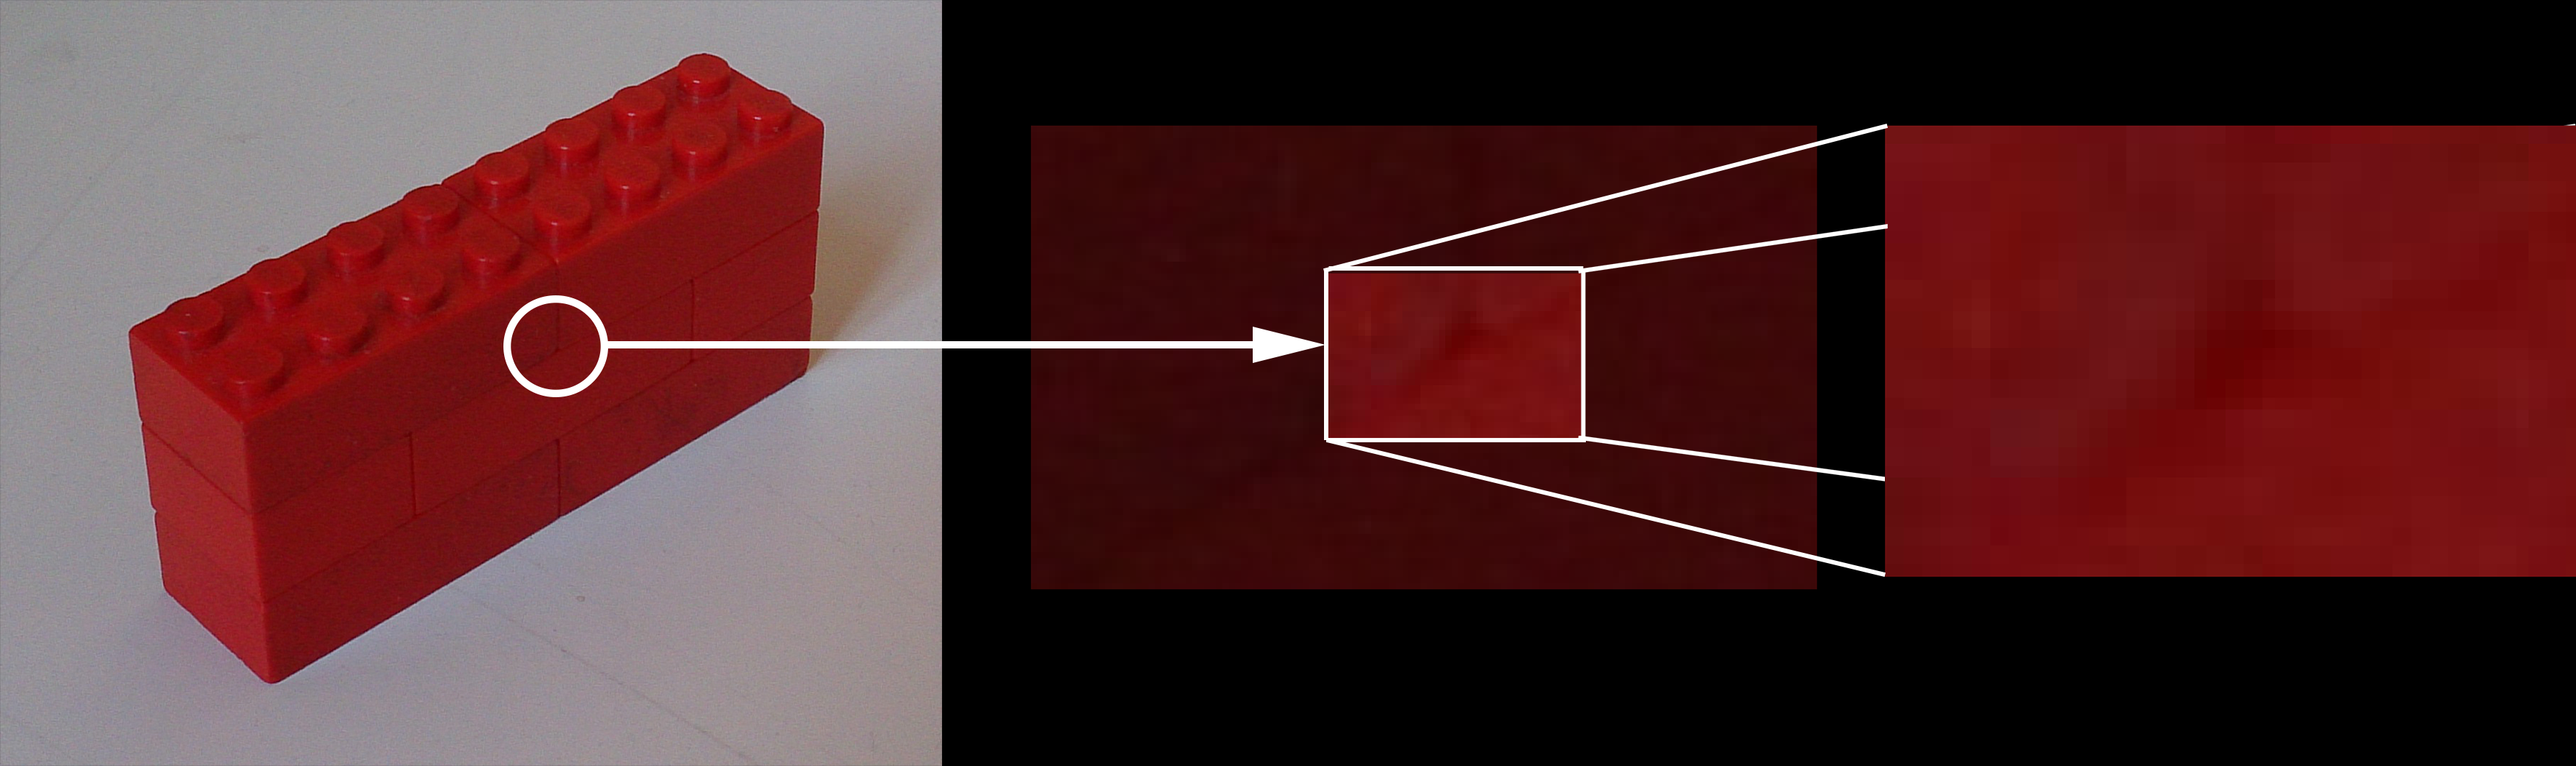
\includegraphics[width=\linewidth]{img/edges}
  \caption{De vergroting van een rand in een muur van legoblokken.}
  \label{fig:besl_edges}
\end{figure}

Hoewel het wel mogelijk is om een enkele legoblok te detecteren is het erg moeilijk om in een constructie van legoblokken de blokken afzonderlijk te detecteren. Dit resulteerde telkens in erg slechte resultaten, zelfs wanneer het beste type feature en de beste classificatie methode werd gekozen. Dit wordt hoofdzakelijk veroorzaakt door de enorme hoeveelheid aan occlusie die een legoblok in een constructie grotendeels verbergt. Hierdoor is slechts een erg beperkt deel van de legoblok (in sommige gevallen slechts \'e\'en vlak, zie figuur \ref{fig:brickWall}) zichtbaar wat het erg moeilijk maakt om met features een legoblok te detecteren. Zelfs indien op voorhand een optimale pose zou worden gekozen kan voor sommige legoblokken enkel \'e\'en vlak zichtbaar zijn in de afbeelding. 

Men zou dan kunnen zeggen dat op basis van de randen de verschillende legoblokken in de constructie kunnen worden gedetecteerd. Dit is echter niet waar omdat deze randen erg zwak zijn wanneer legoblokken met een zelfde kleur naast elkaar staan. Indien we dit probleem van naderbij zouden bekijken bekomen we een resultaat zoals in figuur \ref{fig:besl_edges}. In deze figuur is een deel van de afbeelding dat legoblokranden bevat tweemaal uitvergroot. Deze rand neemt slechts twee \`a drie pixels in beslag en verandert bovendien erg weinig van kleur. Dit maakt het enorm moeilijk, zo niet onmogelijk om de verschillende legoblokken op basis van hun randen te detecteren.

Deze redenering leidt tot een volgend resultaat: het is erg moeilijk, zo niet onmogelijk, om in een legoconstructie alle legoblokken apart te detecteren. Daarom moeten we proberen om, in plaats van de blokken individueel te proberen detecteren, ze als groter geheel te detecteren. Zulke legoconstructie kunnen we zien als een flexibele legoblok die eender welke hoogte, diepte en breedte kan hebben. Dat is exact waarvoor het deformed parts-based feature type gebruikt wordt maar zoals aangehaald in sectie \ref{sec:feat_part} is deze methode te traag om te gebruiken in een mobiele AR applicatie. Dat is de reden waarom in de volgende sectie een sneller alternatief wordt voorgesteld dat gebruik maakt van het idee dat lego constructies moeten gedetecteerd worden in plaats van individuele legoblokken. Hierbij wordt echter wel afgestapt van het idee om CAD modellen te gebruiken.

%Er zijn in een hoofdstuk verschillende onderwerpen. We zullen nu
%veronderstellen dat dit het laatste onderwerp is.

%\subsection{Een item}
%Maak ook geen misbruik van opsommingen. Voor korte opsommingen gebruik je
%geen ``\verb|itemize|'' of ``\texttt{enumerate}'' commando's. Doe dus
%\emph{niet} het volgende:
%\begin{quote}
%  De Eiffeltoren bevat drie verdiepingen:
%  \begin{itemize}
%  \item de eerste;
%  \item de tweede;
%  \item de derde.
%  \end{itemize}
%\end{quote}
%Maar doe:
%\begin{quote}
%  De Eiffeltoren bevat drie verdiepingen: de eerste, de tweede en de derde.
%\end{quote}

%\section{Besluit}
%BESLUIT VAN DIT HOOFDSTUK 
%Als je in dit hoofdstuk tot belangrijke resultaten of besluiten gekomen
%bent, dan is het ook logisch om het hoofdstuk af te ronden met een
%overzicht ervan. Voor hoofdstukken zoals de inleiding en het
%literatuuroverzicht is dit niet strikt nodig.

%%% Local Variables: 
%%% mode: latex
%%% TeX-master: "masterproef"
%%% End: 
